\documentclass[tikz,border=4pt]{standalone}
\usepackage{tikz}
\usepackage{xcolor}
\usetikzlibrary{arrows.meta,calc,decorations.pathmorphing}

\begin{document}
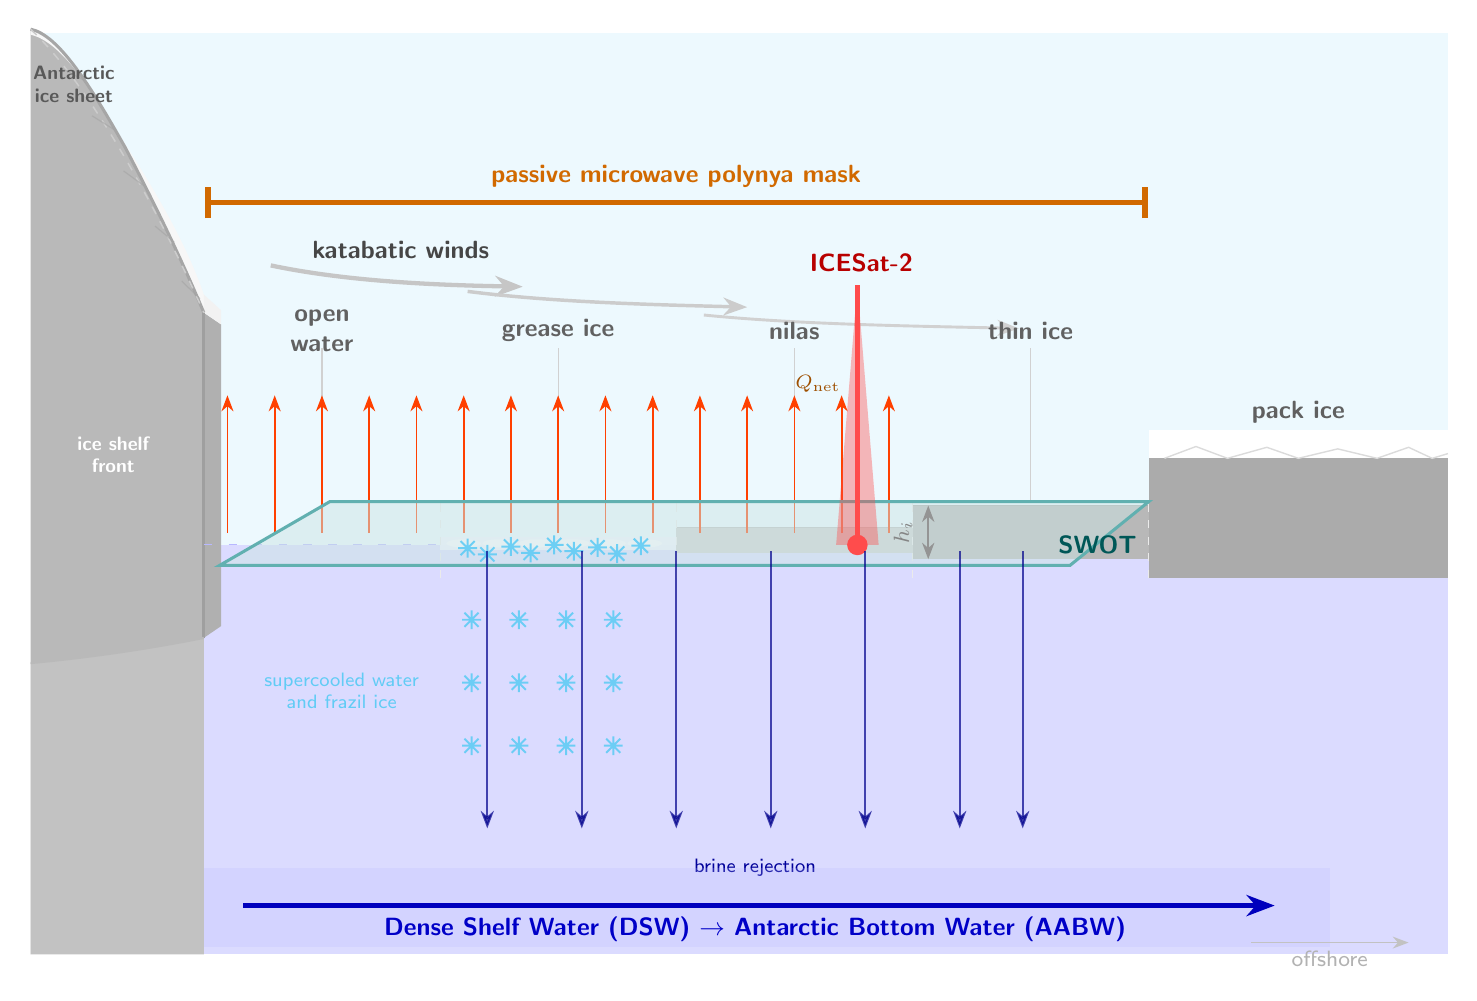
\begin{tikzpicture}[
    font=\sffamily,
    >=Stealth,
    every node/.style={inner sep=2pt},
    frazilstar/.style={draw=cyan!62!white, line width=0.72pt, opacity=0.90}
]
%% ============================================================
%% x: 0-18  |  y: -5.2 to 6.5  |  sea surface at y=0
%% ZONES: ice shelf 0-2.2 | open water 2.2-5.2 | grease ice 5.2-8.2
%%        nilas 8.2-11.2 | thin ice 11.2-14.2 | pack ice 14.2-18.0
%% ============================================================
%% ----- ATMOSPHERE -----
\fill[cyan!7] (0,0) rectangle (18,6.5);
%% ----- OCEAN: single uniform colour -----
\fill[blue!14] (2.2,-5.2) rectangle (18,0);
%% ----- ICE SHEET / ICE SHELF: pronounced downslope to front -----
\path[fill=gray!55]
    (0,-5.2) -- (0,6.55)
    .. controls (0.35,6.48) and (0.75,5.85) .. (1.20,5.05)
    .. controls (1.62,4.25) and (1.95,3.55) .. (2.20,2.95)
    -- (2.20,-1.18)
    .. controls (1.60,-1.30) and (0.85,-1.42) .. (0,-1.50)
    -- cycle;
\path[fill=gray!48]
    (0,-5.2) -- (0,-1.50)
    .. controls (0.85,-1.42) and (1.60,-1.30) .. (2.20,-1.18)
    -- (2.20,-5.2) -- cycle;
\path[fill=white!94!gray]
    (0,6.55)
    .. controls (0.35,6.48) and (0.75,5.85) .. (1.20,5.05)
    .. controls (1.62,4.25) and (1.95,3.55) .. (2.20,2.95)
    -- (2.20,3.18)
    .. controls (1.98,3.82) and (1.58,4.52) .. (1.05,5.32)
    .. controls (0.62,6.05) and (0.28,6.42) .. (0,6.48)
    -- cycle;
\path[fill=gray!62]
    (2.20,2.95) -- (2.42,2.80) -- (2.42,-1.03) -- (2.20,-1.18) -- cycle;
\path[fill=white!90!gray]
    (2.20,2.95) -- (2.42,2.80) -- (2.42,2.98) -- (2.20,3.18) -- cycle;
\draw[gray!70, line width=1.1pt]
    (0,6.55)
    .. controls (0.35,6.48) and (0.75,5.85) .. (1.20,5.05)
    .. controls (1.62,4.25) and (1.95,3.55) .. (2.20,2.95);
\draw[gray!75, line width=1.2pt] (2.20,2.95) -- (2.20,-1.18);
\draw[gray!55, line width=0.8pt]
    (2.20,-1.18) .. controls (1.60,-1.30) and (0.85,-1.42) .. (0,-1.50);
%% Slope emphasis: dashed guide + crevasse texture
\draw[gray!40, dashed, line width=0.55pt]
    (0,6.55) .. controls (0.75,5.85) and (1.62,4.25) .. (2.20,2.95);
\foreach \x/\y/\rot in {0.40/6.05/-28, 0.78/5.45/-32, 1.18/4.75/-36, 1.58/4.05/-40, 1.92/3.35/-44} {
    \draw[gray!72, line width=0.45pt, opacity=0.55]
        (\x,\y) ++(\rot:0.00) -- ++(\rot:0.32);
}
\node[font=\sffamily\scriptsize\bfseries, text=white, align=center]
    at (1.05,1.15) {ice shelf\\front};
\node[font=\sffamily\scriptsize\bfseries, text=gray!70!black, align=center]
    at (0.55,5.85) {Antarctic\\ice sheet};
%% ----- KATABATIC WINDS label -----
\node[font=\sffamily\small\bfseries, text=gray!55!black, align=center]
    at (4.7,3.75) {katabatic winds};
%% ----- PASSIVE MICROWAVE BOUNDARY (raised) -----
\draw[orange!82!black, line width=2.0pt]
    (2.25,4.35) -- (14.15,4.35);
\draw[orange!82!black, line width=2.0pt]
    (2.25,4.15) -- (2.25,4.55);
\draw[orange!82!black, line width=2.0pt]
    (14.15,4.15) -- (14.15,4.55);
\node[font=\sffamily\small\bfseries, text=orange!82!black, align=center,
      fill=cyan!7, inner sep=1.5pt]
    at (8.2,4.68) {passive microwave polynya mask};
%% ----- Near-surface gusts: below PM bracket -----
\draw[->, gray!45, line width=1.55pt]
    (3.05,3.55) .. controls (4.0,3.35) and (5.1,3.30) .. (6.25,3.28);
\draw[->, gray!40, line width=1.25pt]
    (5.55,3.22) .. controls (6.65,3.08) and (7.95,3.05) .. (9.10,3.02);
\draw[->, gray!36, line width=1.05pt]
    (8.55,2.92) .. controls (9.75,2.80) and (11.2,2.78) .. (12.55,2.75);
%% ----- ICE-TYPE LABELS at y=2.72 -----
\node[font=\sffamily\small\bfseries, text=black!62, align=center]
    at (3.7,2.72) {open\\water};
\draw[black!18, line width=0.4pt] (3.7,2.50) -- (3.7,0.55);
\node[font=\sffamily\small\bfseries, text=black!62, align=center]
    at (6.7,2.72) {grease ice};
\draw[black!18, line width=0.4pt] (6.7,2.50) -- (6.7,0.52);
\node[font=\sffamily\small\bfseries, text=black!62, align=center]
    at (9.7,2.72) {nilas};
\draw[black!18, line width=0.4pt] (9.7,2.50) -- (9.7,0.52);
\node[font=\sffamily\small\bfseries, text=black!62, align=center]
    at (12.7,2.72) {thin ice};
\draw[black!18, line width=0.4pt] (12.7,2.50) -- (12.7,0.55);
\node[font=\sffamily\small\bfseries, text=gray!75!black, align=center]
    at (16.1,1.68) {pack ice};
%% ----- SURFACE ICE LAYERS -----
%% Grease ice film (5.2-8.2)
\fill[blue!4!white, opacity=0.92] (5.2,-0.06) rectangle (8.2,0.10);
\foreach \xx in {5.50, 5.96, 6.42, 6.88, 7.34, 7.80} {
    \fill[white, opacity=0.68] (\xx,0.02) ellipse (0.22 and 0.052);
}
%% Nilas (8.2-11.2)
\fill[gray!38] (8.2,-0.10) rectangle (11.2,0.22);
\draw[gray!50, line width=0.4pt] (8.2,0.22) -- (11.2,0.22);
%% Thin ice (11.2-14.2)
\fill[gray!56] (11.2,-0.18) rectangle (14.2,0.50);
\draw[gray!65, line width=0.5pt] (11.2,0.50) -- (14.2,0.50);
%% Pack ice (14.2-18.0) + snow
\fill[gray!66] (14.2,-0.42) rectangle (18.0,1.10);
\fill[white]   (14.2, 1.10) rectangle (18.0,1.46);
\draw[gray!28, line width=0.5pt]
    (14.4,1.10)--(14.8,1.25)--(15.2,1.10)--(15.7,1.24)--
    (16.1,1.10)--(16.6,1.22)--(17.1,1.10)--(17.5,1.24)--
    (17.8,1.10)--(18.0,1.16);
\draw[blue!28, loosely dashed, line width=0.4pt] (2.2,0) -- (5.2,0);
\foreach \xd in {5.2, 8.2, 11.2, 14.2} {
    \draw[gray!16, dashed, line width=0.35pt] (\xd,-0.42) -- (\xd,0.60);
}
%% ----- HEAT FLUX: open water through end of nilas -----
\foreach \xx in {2.5, 3.1, 3.7, 4.3, 4.9, 5.5, 6.1, 6.7, 7.3, 7.9, 8.5, 9.1, 9.7, 10.3, 10.9} {
    \draw[->, orange!50!red, line width=0.62pt] (\xx,0.15) -- (\xx,1.90);
}
\node[font=\sffamily\scriptsize, text=orange!62!black]
    at (10.0,2.05) {$Q_{\mathrm{net}}$};
%% ----- SWOT SWATH -----
\fill[teal!20, opacity=0.50]
    (3.8,0.55) -- (2.4,-0.26) -- (13.2,-0.26) -- (14.2,0.55) -- cycle;
\draw[teal!62, line width=1.1pt]
    (3.8,0.55) -- (2.4,-0.26) -- (13.2,-0.26) -- (14.2,0.55) -- cycle;
\node[font=\sffamily\small\bfseries, text=teal!68!black, align=left]
    at (13.55,0) {SWOT};
%% ----- ICESat-2 TRACK -----
\fill[red!72, opacity=0.38]
    (10.5,3.30) -- (10.23,0.0) -- (10.77,0.0) -- cycle;
\draw[red!70, line width=1.9pt] (10.5,3.30) -- (10.5,0.0);
\fill[red!70] (10.5,0.0) circle (0.13);
\node[font=\sffamily\small\bfseries, text=red!72!black, align=left]
    at (10.55,3.58) {ICESat-2};
\draw[<->, black!42, line width=0.65pt] (11.40,-0.18) -- (11.40,0.50);
\node[font=\sffamily\footnotesize, text=black!48, rotate=90]
    at (11.08,0.16) {$h_i$};
%% =============================================================
%% SUBSURFACE: frazil stars + brine rejection
%% =============================================================
%% Large frazil stars near surface
\foreach \xx/\yy in {
    5.55/-0.04, 6.10/-0.02, 6.65/0.00, 7.20/-0.03, 7.75/-0.01,
    5.80/-0.12, 6.35/-0.10, 6.90/-0.08, 7.45/-0.11
} {
    \draw[frazilstar] (\xx-0.12,\yy) -- (\xx+0.12,\yy)
        (\xx,\yy-0.12) -- (\xx,\yy+0.12)
        (\xx-0.09,\yy-0.09) -- (\xx+0.09,\yy+0.09)
        (\xx+0.09,\yy-0.09) -- (\xx-0.09,\yy+0.09);
}
%% Smaller frazil stars at depth
\foreach \xx/\yy in {
    5.60/-0.95, 6.20/-0.95, 6.80/-0.95, 7.40/-0.95,
    5.60/-1.75, 6.20/-1.75, 6.80/-1.75, 7.40/-1.75,
    5.60/-2.55, 6.20/-2.55, 6.80/-2.55, 7.40/-2.55
} {
    \draw[frazilstar] (\xx-0.12,\yy) -- (\xx+0.12,\yy)
        (\xx,\yy-0.12) -- (\xx,\yy+0.12)
        (\xx-0.09,\yy-0.09) -- (\xx+0.09,\yy+0.09)
        (\xx+0.09,\yy-0.09) -- (\xx-0.09,\yy+0.09);
}
\node[font=\sffamily\scriptsize, text=cyan!62!white, align=center]
    at (3.95,-1.85) {supercooled water\\and frazil ice};
%% Brine rejection arrows
\foreach \xx in {5.8, 7.0, 8.2, 9.4, 10.6, 11.8, 12.6} {
    \draw[->, blue!55!black, line width=0.75pt, opacity=0.70]
        (\xx,-0.08) -- (\xx,-3.60);
}
\node[font=\sffamily\scriptsize, text=blue!60!black]
    at (9.2,-4.10) {brine rejection};
%% DSW / AABW
\fill[blue!28, opacity=0.22] (2.2,-5.10) rectangle (16.5,-4.10);
\draw[->, blue!74!black, line width=1.6pt] (2.7,-4.58) -- (15.8,-4.58);
\node[font=\sffamily\small\bfseries, text=blue!78!black, align=center]
    at (9.2,-4.88)
    {Dense Shelf Water (DSW) $\rightarrow$ Antarctic Bottom Water (AABW)};
%% Offshore indicator
\draw[->, black!24, line width=0.60pt] (15.5,-5.05) -- (17.5,-5.05);
\node[font=\sffamily\footnotesize, text=black!30] at (16.5,-5.26) {offshore};
\end{tikzpicture}
\end{document}
